\chapter{Webbdatabas för hantering av filer}

\section{Systemarkitektur}
I inledningen av projektet hölls en diskussion om hur systemet skulle utvecklas. Faktorer som språk och ramverk togs upp. Beslutet som fattades var att språket Ruby och ramverket Ruby on rails skulle användas som grundstomme i projektet. Vidare användes också Javascript och ramverket Angularjs för att göra upplevelsen av systemet snabbare för användaren.

\subsection{Ruby och Ruby on rails}
Ruby on rails är ett ramverk skrivet i språket Ruby \cite{rubylang}. Det är ett ramverk med öppen källkod som används utav flera stora tjänster på nätet, bland andra mikrobloggstjänsten Twitter, sammarbetsverktyget Github och boendeförmedlingstjänsten Airbnb. Ramverket är skrivet enligt designmönstret MVC. Detta står för \textit{model}, \textit{view}, \textit{controller} och är ett sätt att strukturera ett projekts logik på sådant vis att olika komponenter har sin egna tydliga plats och syfte.

I Ruby on rails skapar utvecklaren \textit{models}. Detta är en samling klasser vars syfte är att hantera data som användaren eller systemet interagerar med, och fungerar som ett lager ovanpå databasen. Ett exempel på en \textit{model} kan vara en klass för användare eller filer. Genom dessa klasser hanteras all information om just användare respektive filer, och samtliga databasoperationer sker genom klassernas metoder.

Den komponent som sköter interaktionen mellan användare och systemets \textit{models} är systemets \textit{controllers}. Här finns logik för att hantera användares handlingar och hämta data från systemets \textit{models}. Ett exempel kan vara att användaren klickar på en knapp i webbläsaren. Syftet med knappen är att visa en viss data. Användarens handling skickas till en \textit{controller} som tar emot vad det är för data som användaren efterfrågar och hämtar den datan från en \textit{model}. Här kan också logik för att hantera undantag, till exempel att datan saknas, finnas. Den \textit{controller} som anropats skickar sedan resultatet av användarens begäran vidare till användaren.

Det som användaren i sin tur interagerar med är systemets \textit{views}, på svenska vyer. Här presenteras det som systemets \textit{controllers} producerat. Knappen som användaren trycker på i exemplet i stycket ovan skapas i en \textit{view}. Här kan också finnas länkar, texter, textfält och alla andra komponenter som utgör det som renderas av en webbläsare.

En mer överskådlig figur för hur data och interaktioner generellt sett färdas genom ett MVC-system visas i figur \ref{fig:mvc1}. Data transporteras från \textit{models} till \textit{views} via \textit{controllers}. Interaktioner färdas mellan \textit{views} och \textit{models} via \textit{controllers} och direkt mellan \textit{controllers} och \textit{views} samt mellan \textit{controllers} och \textit{models}.

\begin{figure}[!H]
\centering
\includegraphics[width=0.8\textwidth]{figures/mvc1.png}
\caption{Visar på dataflödet i ett MVC-system}
\label{fig:mvc1}
\end{figure}

En annan figur som snarare fokuserar på MVC ur ett användarperspektiv visas i figur \ref{fig:mvc2}.

\begin{figure}[!H]
\centering
\includegraphics[width=0.8\textwidth]{figures/MVC_wiki.png}
\caption{Visar på MVC-flödet ur ett användarperspektiv.}
\label{fig:mvc2}
\end{figure}

Fördelarna med att använda ett webbramverk som Ruby on rails eller motsvarande är flera, och kan generaliseras med att säga att det är onödigt att uppfinna hjulet på nytt. Säkerhet, effektivitet och struktur är aspekter som förstärks utav Ruby on rails. En mer konkret fördel med Ruby on rails är klassen \emph{ActiveRecord} som alla modeller i systemet ärver av. \emph{ActiveRecord} har funktioner för att hantera relationer och frågor mot databasen. Mer om \emph{ActiveRecord} och databashantering i kapitel \ref{ssec:activerec}.

\subsection{Javascript och Angularjs}
För att skapa ett responsivt system, i bemärkelsen att det var snabbt för användaren, valdes det att implementera mycket utav funktionaliteten hos klienten med hjälp av Javascript. Systemet innehåller många olika komponenter som ska interagera med varandra. Ett exempel är då flera filer ska listas med verktyg för att hantera filen, samtidigt som den filen har flera taggar som också ska kunna hanteras.

Ramverket Angularjs valdes bland annat på grund av dess stöd för så kallade templates men även för dess tvåvägsbindning för variabler. Tvåvägsbindningen gjorde det enklare att utveckla komponenter som beror på hur användaren interagrerar med textfält eller knappar. Till exempel krävdes det väldigt lite ansträngning för att uppdatera en rubrik till det som användaren skrev i ett textfält samtidigt som denne skrev, eller att uppdatera både textfältet och rubriken samtidigt.

Angularjs är ett så kallat MVW-ramverk, vilket står för \textit{Model-View-Whatever} \cite{angularjs}. För att effektivt använda detta ramverk bör även systemet byggas upp efter den designen. Då \textit{whatever} innebär att det finns flera olika typer av sätt att kontrollera eller manipulera data på kan varje komponent i systemet få specialanpassade lösningar.

\section{Tredjepartsmjukvara}
Då Ruby on rails och Angularjs är mjukvara med öppen källkod har det bildats globala nätverk kring dessa ramverk. Många tillägg, verktyg och bibliotek har skrivits för att underlätta utvecklandet i dessa ramverk. För att fortsätta bidra till detta nätverk utvecklades även projektet med hjälp av öppen källkod, för att kunna dela de lösningar som tagits fram.

För att underlätta för utvecklare har Ruby on rails byggts med många verktyg för utvecklare. Möjligheten finns även för utvecklare att bygga egna verktyg som kallas för \textit{gems} och är ofta fria att använda och även de är skrivna med öppen källkod. Några som använts under utvecklandet av detta system är:

Byebug, ett avlusningsverktyg som möjliggör för utvecklare att sätta brytpunkter i koden. När systemet kör och stöter på den rad där denna brytpunkt finns pausas systemet. I konsolen kunde sedan variabler granskas och utvecklarna kunde steg för steg följa vilken väg koden följde.

Letter opener, ett verktyg för att hantera e-post som skickas av systemet. Istället för att utvecklaren sätter upp en e-postserver som skickar e-postmeddelandena på riktigt öppnar Letter opener mailen i webbläsaren. Detta gjorde att utvecklingen av systemets e-postrelaterade komponenter blev betydligt enklare.

För utvecklandet av Angularjs och annan Javascript användes Chrome developer tools och tillägget Angularjs batarang. Dessa är verktyg som gör det lättare för utvecklare att följa med i vad som händer då de använder webbläsaren Google chrome. Med funktioner som brytpunkter och möjligheten att bevaka variabler blir utvecklandet betydligt enklare.

\section{Filhantering}
För att hantera tjänstens filer implementerades tre olika fillagringssätt. En modulär filhantering skapades för att lätt kunna implementera fler sätt att lagra filer. Dropbox implementerades först eftersom det ansågs vara ett enkelt sätt att hantera användarens filer. När det väl implementerats upptäcktes det att Dropbox krävde en krypterad anslutning till systemet, vilket kostar pengar. På grund av detta infördes även Google drive som lagringssätt. Efter ett möte med kunden flyttades fokus till att också implementera lokal fillagring.

\subsection{Dropbox}
Dropbox implementerades med hjälp av Dropbox SDK. SDK står för \textit{Software Development Kit} vilket är en uppsättning av utvecklingsverktyg för mjukvaruutveckling mot specifika ramverk eller programpaket, i det här fallet till utveckling mot Dropbox tjänster. Dropbox SDK ger verktyg för att utveckla nya tjänster som använder sig av Dropbox olika funktioner. Webbtjänsten som utvecklades använder sig av ned- och uppladdning av filer till och från Dropbox. För att nå användarens filer måste en autentisering till Dropbox ske, vilket görs med hjälp av Omniauth, en \textit{gem}. Med hjälp av Dropbox SDK hämtas metadata för filerna i rot-mappen för att sedan visas för användaren. Om en mapp sedan blir klickad på hämtas metadatan för filerna i den mappen med hjälp av sökvägen. En fil laddas också ned med hjälp av dess sökväg. För att ladda upp filer till Dropbox krävs det att de läggs till i en existerande mapp eller i rot-mappen. För att hålla filerna som laddats upp från tjänsten till Dropbox samlade, skapades först en mapp i Dropbox dit filerna laddades upp till.

\subsection{Google drive}
Likt Dropbox användes Google drives SDK för att kunna använda deras funktionalitet i systemet. För att nå användarens filer krävs en autentisering för att ansluta till användarens konto hos Google drive. Det här görs med hjälp av två \textit{gems}, Drive SDK samt Omniauth. Filhanteringen sker likt metoden för Dropbox förutom att Drive inte strukturerar sina filer med hjälp av sökvägar. Varje fil har istället en parameter för \textit{parent} och varje mapp har en parameter \textit{child}, där eventuella filer i mappen lagras. Om en fil ligger i en mapp är mappen filens \textit{parent} och filen är mappens \textit{child}. För att identifiera det här förhållandet kommer alla filer som ligger i samma mapp ha mappens id i dess \textit{parent} parameter. Liknande kommer mappens parameter \textit{child} innehålla alla id tillhörande filer som ligger i mappen, se figur \ref{fig:parentchild}.

\begin{figure}[!H]
\centering
\includegraphics[width=0.8\textwidth]{figures/parentchild.png}
\caption{Visar strukturen för parametrarna \textit{parent} och \textit{child} i Google drive.}
\label{fig:parentchild}
\end{figure}

\subsection{Lokal fillagring}
Den lokala filhanteringen infördes för att ge användaren ett alternativ utan extern kostnad och utan filutrymmesbegränsningar från externa tjänster. För att sköta uppladdningen, som är en central del av den lokala filhanteringen i och med att det inte går att importera filer likt från Google drive eller Dropbox, implementerades en så kallad drag och släpp-uppladdning. Detta innebär att användaren kan markera en eller flera filer på sin dator, och dra dem till webbläsarfönstret där systemet är öppet, och släppa dem där. Systemet tar där vid och laddar upp filerna. När servern har tagit emot all uppladdningsdata från webbläsaren får filen ett slumpat filnamn och placeras i en mapp på servern.

\section{Hantering och strukturering av databaser}
Systemet använder sig utav en SQL-databas, där SQL står för \textit{Structured Query Language}. Det är ett programmeringsspråk för att lagra, bearbeta och hämta information i en databas \cite{sqlenc}.

\subsection{Databasstruktur}
\label{ssec:activerec}

\subsection{Databashantering}

\section{Gränssnitt}

\section{Testning}

\section{Utvecklingsmetodik}

\subsection{Sprint 1 - MVP}

\subsection{Sprint 2 - Utveckla den tekniska funktionaliteten}

\subsection{Sprint 3 - Tänka på användaren}

\subsection{Sprint 4 - Färdig produkt}

\section{Versionshantering och kodgranskning}
